\documentclass{note}

\title{MB Note}
\author{}

\begin{document}
\maketitle
\thispagestyle{fancy}

\vspace{-10pt}

\section{Dinamical Systems}

\subsection{Models of Biological Systems}

\begin{MyTh}{Logistic Growth Model (Population)}
    \ok{Model}: $\frac{dN}{dt}=rN(1-\frac{N}{K})$ \quad {\scriptsize \comment{N}: population at time $t$; \comment{K}: carrying capacity \ps{(depends on resources)}; \comment{r,K}: $>0$.}

    \vspace{-2pt}
    {\footnotesize \quad \ok{Sol}: $N(t)=\frac{N_0Ke^{rt}}{K+N_0(e^{rt}-1)}\stackrel{\infty}{\to}K$ \qquad \ok{Equilibrium points}: $N=0$ (unstable), $N=K$ (stable). \qquad \ok{Quickest:$N=\frac{K}{2}$} \ps{(<:凹; >:凸)}}
\end{MyTh}

\begin{MyTh}{Delay Model}
    \ok{Model}: $\frac{dN}{dt}=f(N(t),N(t-T))$ \quad {\scriptsize \comment{T}: delay time $> 0$ \quad \comment{\scriptsize 周期解|与初始值无关}} \quad \ps{ps: To consider e.g. gestation period, maturation time etc.}

    {\scriptsize \quad \ok{$^1$Ext. of Logistic Model}: $\frac{dN}{dt}=rN(t)\left[1-\frac{N(t-T)}{K}\right]$ \ps{\tiny (用"ave. pop."估计,准用"Convolution Type")}  \ $\Rightarrow$ \ \ok{$^2$Dimensionless}: $\frac{dN^*}{dt^*}=N^*(t^*)\left[1-N^*(t^*-T^*)\right]$ \ps{\tiny ($N^*=\frac{N}{K}, t^*=rt, T^*=rT$)}}

    {\scriptsize \quad \ok{$^{1,2}$} \ok{Periodic sol}: stable limit cycle $N(t+t_p)=N(t)$, $t_p$: period. \ok{Amplitude}: $rT$ \ok{Equilibrium Points}: $N=0|N^*=0$ {\tiny (unstable)}; $N=K|N^*=1$ {\tiny (Stable: $0<T^*=rT<\frac{\pi}{2}$; Unstable: $T^*>\frac{\pi}{2}$)}}
\end{MyTh}

\begin{MyTh}{Continuous Population Model {\scriptsize (EN)}}
    \ok{Model}: $\frac{dN}{dt}=rN(1-\frac{N}{K})-EN=f(N)$ \quad {\scriptsize \comment{r,K,E}: $>0$; \comment{EN}: harvesting rate/unit time; \comment{E}: effort measure.}

    {\scriptsize \quad \ok{Equilibrium}: $N=0$ {\tiny (unstable)}; $N=N_h(E)=K(1-\frac{E}{r})>0$ {\tiny \ps{(need $E<r$, Stable)}} \ok{Yield}: $Y(E)=EN$ \ \ $\cdot$ \ok{$E>r$}:die out; else: \ok{Max Yield}: $Y_M=\frac{rK}{4}$ {\tiny ($E=\frac{r}{2}$)} \ok{Steady State}: $N_{h|Y_M}=\frac{K}{2}$}
\end{MyTh}

\begin{MyTh}{Continuous Population Model {\scriptsize ($Y_0$)}}
    \ok{Model}: $\frac{dN}{dt}=rN(1-\frac{N}{K})-Y_0=f(N;r,K,Y_0)$ \quad {\scriptsize \comment{$Y_0$}: constant yield rate/unit time.}

    {\scriptsize \quad \ok{Max Yield}: $Y_M=\frac{rK}{4}$ \quad \ok{Equilibrium}: $^1$$0<Y_0<Y_M$: Two positive points \ps{(unstable(小) and stable(大))}. \ \ \ok{Sensitivity}: {\tiny 对于fluctuation此模型和EN模型都不稳定,但此模型更敏感sensitive.}}
\end{MyTh}

\begin{MyTh}{Examples of $N_{t+1}=f(N_t)$}
    \ok{Verhulst}: $N_{t+1}=rN_t(1-\frac{N_t}{K});r,K>0$. \ \ Better: \ok{Ricker curve}: $N_{t+1}=N_t e^{r(1-\frac{N_t}{K})}$
\end{MyTh}

\begin{MyTh}{Imperfect Bifuraction}
    $\dot{x}=rx-x^3+h$ \scalebox{0.8}{\ps{\tiny (codimension-2 bifuraction)}} \ \ \scalebox{0.8}{\tiny If $r\leq0$, $x^*$ unique. If $r>0$, $|h|>h_c$, $x^*$ unique; $|h|<h_c$, $x^*$ three. (两边stable,中unstable). Bifuraction points: $h=\pm h_c=\pm\frac{2r}{3}\sqrt{\frac{r}{3}}$. \ \textbf{cusp point}: $(r,h)=(0,0)$}
\end{MyTh}


\subsection{Summary - Stability and Bifuraction}

{\tiny
\begin{tabular}{|@{\hskip 2pt}c@{\hskip 2pt}||l|l|l|l||l|l|l|l|}
    \hline
    & \multicolumn{4}{c||}{$\frac{dN}{dt}=f(N)$ \quad \ok{No Limit cycle periodic solutions} \qquad $S$: stable; $U$:unstable.} & \multicolumn{4}{c|}{$N_{t+1}=N_tF(N_t)=f(N_t)$ \quad \ok{Eigenvalue}: $\lambda=f'(N^*)$} \\
    \hline
    Stability & \multicolumn{2}{l|}{Stable: $f'(N^*)<0$} & \multicolumn{2}{l||}{Unstable: $f'(N^*)>0$} & Stable: $|\lambda|<1$ & Unstable: $|\lambda|>1$ \scalebox{0.8}{\ps{(chaotic)}} & \multicolumn{2}{l|}{Periodic: $|\lambda|=1$ \scalebox{0.8}{$\begin{cases}+:\text{tangent bifurcation} \\ -:\text{period-doubling bifurcation}\end{cases}$} \hspace{-8pt} \scalebox{0.9}{\ps{\tiny (neutrally stab.)}}} \\
    \hline
    \ok{Linearise} & \multicolumn{4}{l||}{$N(t)=N^*+n(t), |n(t)|\ll1$ \ $\Rightarrow$ \ $\frac{dn}{dt}=\frac{dN}{dt}=$\scalebox{0.8}{$\begin{cases}\text{\ps{(general)}}=f(N^*)+f'(N^*)n(t) \\ \text{\ps{(delay)}=直接带入f后近似}\end{cases}$}} & \multicolumn{4}{l|}{Let $N_t=N^*+n_t, |n_t|\ll1$ \ $\Rightarrow$ \ $N^*+n_{t+1}=\cdots=f(N^*+n_t)\approx f(N^*)+f'(N^*)n_t$ \ $\Rightarrow$ \ $n_{t+1}=\lambda n_t$} \\
    \hline
    \multirow{2}{*}{\scalebox{0.9}{\makecell{Bifuraction \backslash\backslash \\ Perturbations \\ at $N^*$ | Periodic}}} & \multirow{2}{*}{\makecell{\scalebox{0.8}{Saddle-Note} \scalebox{0.7}{\ok{(Normal Form)}} \\ $\dot{x}=r\pm x^2$ \\ 0$\to$S$\to$U-S}} & \multirow{2}{*}{\makecell{Transcritical \\ $\dot{x}=rx-x^2$ \\ S-U$\to$U-S}} & \multirow{2}{*}{\makecell{\scalebox{0.9}{(super-)Pitchfork} \\ $\dot{x}=rx-x^3$ \\ S$\to$S-U-S}} & \multirow{2}{*}{\makecell{\scalebox{0.9}{Sub-critical Pitchfork} \\ $\dot{x}=rx+x^3$ \\ U$\to$U-S-U}} & $\lambda<-1$: $\uparrow$ oscillations & $-1<\lambda<0$: $\downarrow$ oscillations & $0<\lambda<1$: $\downarrow$ Monotone & $\lambda>1$: $\uparrow$ Monotone \\
    \cline{6-9}
    & & & & & \multicolumn{4}{l|}{If $f^p(N^*)=N^*$, $N^*$ is $p$-periodic. \quad | \quad $\forall$ even $p$-periodic $N^*$ with $\lambda=-1$ branches into $2p$-periodic} \\
    \cline{6-9}
    & & & & & \multicolumn{3}{l|}{\textbf{Sarkovskii's Theorem}: If a $3$-periodic $N^*$ exists, then $\forall p\ge1$, $p$-periodic $N^*$ exists.} & \scalebox{0.9}{\ok{Species extinction}: $N_{\min}<1$} \\
    \hline
    Other & \multicolumn{4}{l||}{\textbf{Time-Independent}: At $N^*$: \ok{$\frac{dN}{dt}=0$} \ \ \ok{$N(t)=N(t-T)=N^*$} \ \ \ok{$f(N^*)=0$}} & \multicolumn{4}{l|}{\ok{Max/Min}: \scalebox{0.8}{\ps{[如果单峰(unimodal)|2-periodic]}} $f'(N_m)=0$, $N_{\max}=f(N_m)$ \ ; \ $N_{\min}=f(N_{\max})$ \ \ \scalebox{0.8}{\tiny $\downarrow$ $E,Y_0$对应两种模型}} \\
    \hline
    Other & \multicolumn{8}{l|}{\ok{Tangency Condition}: If $\dot{x}=f(x,r)$, 分岔点 $(x^*,r_c)$: \ok{$\frac{\partial f}{\partial x}|_{(x^*,r_c)}=0$ \ \ $f(x^*,r_c)=0$} \quad | \quad 两点合并:\imp{coalesce}. \qquad || \qquad \imp{Recovery Time}: \ok{$T=-\frac{1}{\lambda}$} \scalebox{0.9}{\ps{\tiny 比收获模型好 \ 看recovery time} $\to$ 算$\frac{T(E)}{T(0)}$|$\frac{T(Y)}{T(0)}$ 小好}} \\
    \hline
\end{tabular}
}

\vspace{-2pt}
\begin{MyTh}{Hopf Bifuraction}
    {\scriptsize \ps{平衡点从稳定变为不稳定，同时产生 limit cycle}. 条件: $\det(J)>0$; $\frac{d\text{tr}(J)}{d\mu}\ne0$ \ps{or: $\text{tr}(J)$ +/-符号有变化} \ \ $\Leftrightarrow$ \ \ $\lambda=\pm iw$ and $\frac{d\Re(\lambda)}{d\mu}\ne0$ \quad \ps{$\mu$: parameter, not time.}}

    {\scriptsize \quad $\Rightarrow$ Stable $\to$ Unstable + Stable Limit Cycle \ps{\tiny (supercritical)} \ \ or \ \ Unstable $\to$ Stable + Unstable Limit Cycle \ps{\tiny (subcritical)}. \ \ \ps{\tiny (一般super-)} \quad when $\text{tr}(J)=0|\Re(\lambda)=0$, $\lambda=\pm iw$ $\Rightarrow$ \ok{periodic}: $T=\frac{2\pi}{w}$}
\end{MyTh}


\begin{MyTh}{Bifuraction}
    Qualitative changes in dynamics are called \textit{bifuractions}. \imp{\tiny (当平衡点性质|个数发生变化时)} \quad \ok{Bifuraction Diagram}: {\tiny y轴:平衡点; x轴:控制参数; 虚线unstable,实线stable.}
\end{MyTh}

\begin{MyTh}{稳定性Stability判别|For Continuous Model}
    Find perturbation: $n(t)$ and $\frac{dn}{dt}$ \ $\Rightarrow$ \ Assume $n(t)=e^{\lambda t}|ce^{\lambda t}$ \ $\to$ \ Find $\lambda=g(\lambda)$ \ $\Rightarrow$ \ Let $\lambda=u+iw$ $\to$ $u=g_1(u)$ and $w=g_2(w)$ \ $\Rightarrow$ \ $u<0$ asy.stable; $u>0$ unstable. \quad \imp{Find $T_c$}: \ps{\tiny (如要寻找 参数(e.g. $T$) 范围/临界值 \ 使得平衡点稳定)} Check $T=0$ stable. $\Rightarrow$ Using $u=0$ \ps{\tiny (i.e. $\lambda=iw$)} to find $T_c$.
\end{MyTh}

\section{Interacting Populations}

\begin{MyTh}{Lotka-Volterra Model {\tiny (Predator-Prey)}}
    $\frac{dN}{dt}=N(a-bP); \frac{dP}{dt}=P(cN-d)$ \ $\Rightarrow$ \ nondim: $\frac{du}{d\tau}=u(1-v); \frac{dv}{d\tau}=\alpha v(u-1)$ \quad \ok{Equilibrium}: $(u^*,v^*)=(0,0),(1,1)$

    {\footnotesize \quad \ok{Exact sol}: $\alpha u+v-\ln(u^\alpha v)=H$, $H>H_{min}=\alpha+1$ constant. \ \ \ps{\tiny (closed phase)}  \ \ \ok{Conservation Law}: Using $\frac{du}{dv}=\frac{du}{d\tau}\frac{d\tau}{dv}$ find $H$ \ $\Rightarrow$ \ $\frac{dH}{d\tau}=0$, here it satisfies.\ \ps{\tiny (By chain rule)}}

    {\footnotesize \quad \ok{Show Level curves \ps{\tiny (constant of motion)} closed}: If $H(u,v)$ is level curve, Look $\left[\begin{smallmatrix}H_{uu} & H_{uv} \\ H_{vu} & H_{vv}\end{smallmatrix}\right]_{(u^*,v^*)}$ $\Rightarrow$ If $+/-$ definite (i.e. $\forall\lambda_i>0(<0)$) \qquad $\uparrow$ \ps{\tiny 轨迹会在level curve$\to$oscillation}}

    \vspace{-3pt}
    {\footnotesize \quad\qquad $\Rightarrow$ It's local min/max at $(u^*,v^*)$ \& strictly convex/concave $\Rightarrow$ closed curves. \qquad \ps{Closed curves $\Rightarrow$ periodic sol.}}
\end{MyTh}

\begin{MyTh}{Determinant Stability}
    \scriptsize
    For model: $\left[\begin{smallmatrix}u'(t) \\ v'(t)\end{smallmatrix}\right]=\left[\begin{smallmatrix}f(u,v) \\ g(u,v)\end{smallmatrix}\right]${\tiny at equilibrium $(u^*,v^*)$}. Let $\left[\begin{smallmatrix}x \\ y\end{smallmatrix}\right]=\left[\begin{smallmatrix}u-u^* \\ v-v^*\end{smallmatrix}\right]$, then $\left[\begin{smallmatrix}x' \\ y'\end{smallmatrix}\right]=\left[\begin{smallmatrix}f_u & f_v \\ g_u & g_v\end{smallmatrix}\right]_{(u^*,v^*)}\left[\begin{smallmatrix}x \\ y\end{smallmatrix}\right]$
    \ \ $\Rightarrow$ \ \ Find eigenvalues $\lambda$ of $J$ by $\det(J-\lambda I)=0$

    \quad $^1$ $\det(J)>0, \text{tr}(J)<0$ $\Leftrightarrow$ $\Re(\lambda)<0$ $\rightarrow$ stable node \scalebox{0.7}{\ps{\tiny $Im(\lambda)=0$}}; stable focus=spiral point \scalebox{0.7}{\ps{\tiny $Im(\lambda)\ne0$}}; $^2$ $\det(J)>0, \text{tr}(J)>0$ $\Leftrightarrow$ $\Re(\lambda)>0$ $\rightarrow$ unstable node \scalebox{0.7}{\ps{\tiny $Im(\lambda)=0$}}; unstable focus=spiral point \scalebox{0.7}{\ps{\tiny $Im(\lambda)\ne0$}}

    \quad $^3$ $\det(J)<0$ $\Leftrightarrow$ $Im(\lambda)=0$, $\lambda_1<0<\lambda_2$ $\rightarrow$ saddle point (unstable); $^4$ $\det(J)>0, \text{tr}(J)=0$ $\Leftrightarrow$ $\lambda=\pm iw$ (pure imaginary) $\rightarrow$ center \ps{\tiny (only linear stability)}|Hopf bifurcation (见前面)

    \quad \ok{Nullclines}: $f(u,v)=0$ or $g(u,v)=0$ \ $\to$ \ {\tiny 得u,v表达线条是nullclines.}
    \quad \ok{Trapping Region}: {\tiny A closed region $R$ \tiny{可以用直线/null clines构成} \ \ s.t. \ \ 所有 \ 边界的\textit{外}法线方向$\mathbf{n}$, 在对应边界上的点, 满足$\mathbf{n}\cdot\left[\begin{smallmatrix}f(u,v) \\ g(u,v)\end{smallmatrix}\right]<0$}

    \vspace{-2pt}
    \quad \ok{Find slope of Nullclines}: $f(u,v)=0$ $\Rightarrow$ $df=f_u du+f_v dv=0$ $\Rightarrow$ $\frac{dv}{du}=-\frac{f_u}{f_v}$ \qquad Similarly: $\frac{dv}{du}=-\frac{g_u}{g_v}$\hspace{100pt}$\uparrow$ \ps{\tiny 也叫 bounding region (confined region)}
\end{MyTh}

\begin{MyTh}{Poincare-Bendixson Theorem}
    One unstable node/focus/spiral point + it's in \textit{trapping region} $\Rightarrow$ A \ok{stable limit cycle} exists. \ \ \ps{\tiny (Cannot be a saddle (since $\det(J)$ cannot be $<0$))}
\end{MyTh}

\begin{MyTh}{Competition Model}
    \ok{principal of competitive exclusion}: {\tiny If two species compete for the same limited resource, one will eventually outcompete and exclude the other.} \ps{\tiny (b,c,d; $b$ 物种谁最后存活取决于初始值)}
\end{MyTh}

\begin{minipage}{0.75\textwidth}
    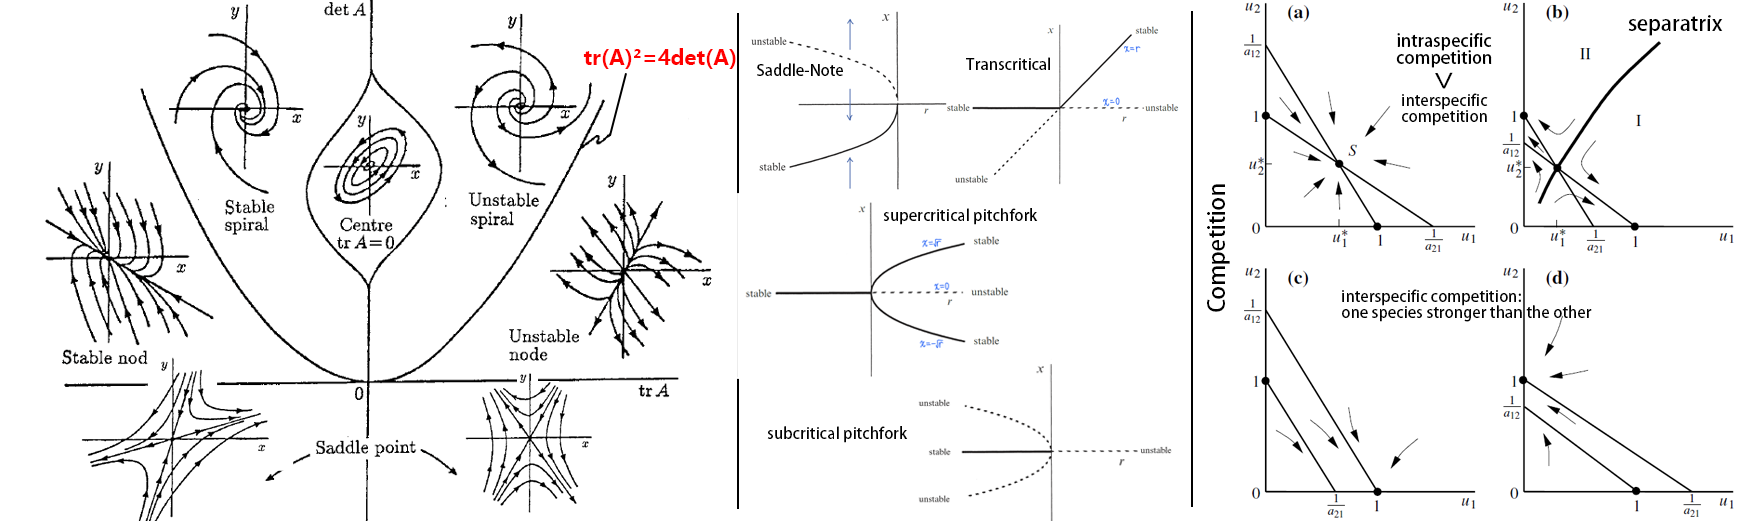
\includegraphics[width=1\textwidth]{graph1.png}
\end{minipage}
\hfill
\begin{minipage}{0.25\textwidth}
    \begin{MyTh}{Mutualism|Symbiosis}(共生)

        {\tiny Case I: 图(a) \ps{coexist: competition not aggressive.}}

        {\tiny Case II: 两条射线 \ps{both species grow unboundedly.(all unstable)}}

        {\tiny Case II: 两条向外的线相交在一点 \ps{both species tend to a stable coexistence.}}
    \end{MyTh}

    \begin{MyTh}{For small perturbations}
        \scriptsize If fixed point is \ok{Center} or \ok{Imporper Node} (GM=1): Any small perturbation $\Rightarrow$ may change to spiral point. $\Rightarrow$ Not structurally stable.
    \end{MyTh}

    \begin{MyTh}{Chaotic}
        \scriptsize Three dim or delay $\Rightarrow$ 可能 chaotic.
    \end{MyTh}

    \begin{MyTh}{Limit Cycle}
        \tiny Any sufficiently perturbation from a stable limit cycle $\Rightarrow$ trajectory returns to the limit cycle. (i.e. tends to zero asymptotically with time)
    \end{MyTh}
    \vspace{-10pt}
\end{minipage}


\section{Reaction Kinetics}

\vspace{-5pt}
\begin{MyTh}{Enzyme Kinetics}
    {\footnotesize e.g. $S+E\underset{k_{-1}}{\stackrel{k_1}{\rightleftharpoons}}SE\stackrel{k_2}{\rightarrow}P+E$} \quad \comment{$K_i$}: rate of reaction; \comment{$S$}: substrate; \comment{$E$}: enzyme; \comment{$SE$}: complex; \comment{$P$}: product. \quad \ok{Rate of uptake}: $v=\frac{d[P]}{dt}|_{t=0}$
\end{MyTh}

\vspace{-8pt}
\begin{MyTh}{Law of Mass Action}
    \tiny Rate of reaction is proportional to the product of the concentrations of the reactants. \ \ \ps{\tiny e.g. $\alpha_1 A+\alpha_2 B\underset{k_{-1}}{\stackrel{k_1}{\rightleftharpoons}}\beta_1 C+\beta_2 D$ \ $\Rightarrow$ \ $\text{rate}_{\text{forward}}=k_1[A]^{\alpha_1}[B]^{\alpha_2}$; $\text{rate}_{\text{backward}}=k_{-1}[C]^{\beta_1}[D]^{\beta_2}$}
\end{MyTh}

\vspace{-5pt}
\begin{MyTh}{Quasi-Steady State Approximation (QSSA)}
    \tiny 如果系统里有\textit{快}和\textit{慢}变量, 则可以假设\textit{快}变量达到稳态, 即 $\frac{d(\text{fast})}{dt}=0$. \ps{\tiny (or $\eps\to0$; 一般来说假设 complex concentration changes rapidly)}
\end{MyTh}

\begin{MyTh}{Singular Perturbations Analysis}
    For $\frac{du}{d\tau}=f(u,v)$, $\eps\frac{dv}{d\tau}=g(u,v)$, $0<\eps\ll1$ \ $\Rightarrow$ \ $v$ fast \ps{\tiny (when $g\not\to0$)}, $u$ slow. \ \ {\scriptsize \ok{Quasi-steady-state approximation}: $\eps\to0$ $\Rightarrow$ $g(u,v)=0$}

    \vspace{-3pt}
    {\footnotesize \quad \ok{Taylor: $u(\tau,\eps)=\sum\limits_{n=0}^\infty \eps^n u_n(\tau)$; $v(\tau,\eps)=\sum\limits_{n=0}^\infty \eps^n v_n(\tau)$}} \quad \ok{Outer solution}: {\scriptsize Taylor带入原方程组$\to$保留$\Ocal(1)|\eps=0$} \ \ \ps{\tiny Valid for $\tau>0$ (slow time); $v_0(0)$ \imp{unvalid}.$\to$not uniformly valid for $\tau\geq0$}
    
    \vspace{-3pt}
    {\footnotesize \quad \ok{Inner solution}: $\sigma = \frac{\tau}{\eps}$, $\begin{smallmatrix}U(\sigma;\eps)=u(\tau;\eps) \\ V(\sigma;\eps)=v(\tau;\eps)\end{smallmatrix}$ $\Rightarrow$ $\frac{dU}{d\sigma}=\eps f(u,v)$, $\frac{dV}{d\sigma}=g(u,v)$ $\to$ {\scriptsize Taylor 带入原方程组$\to$保留$\Ocal(1)|\eps=0$} \ps{\tiny (known as \ok{boundary layer} ($\tau=0$处)); Valid $\tau=0$ (fast time)}}

    {\footnotesize \quad \ok{Asymptotic Matching}: {\scriptsize $\lim\limits_{\sigma\to\infty}[U_0(\sigma),V_0(\sigma)]=\lim\limits_{\tau\to0^+}[u_0(\tau),v_0(\tau)]$} \qquad \ok{Uniformly Valid Solution}: {\scriptsize $u(\tau;\eps)=u_0(\tau)+\Ocal(\eps)$; $v(\tau;\eps)=\left\{ \begin{smallmatrix} v_0(\tau)+\Ocal(\eps), & 0<\eps\ll \tau \\ V_0(\sigma)+\Ocal(\eps), & 0<\tau\ll 1 \end{smallmatrix}\right.$} \tiny \ok{uniform expansion}: 见chp.5}
\end{MyTh}

\vspace{-3pt}
\begin{MyTh}{Activator-Inhibitor Model}
    For $\frac{du}{dt}=f(u,v)$, $\frac{dv}{dt}=g(u,v)$: If $\frac{\partial g}{\partial u}>0$, $u$ is an \ok{activator} of $v$; If $\frac{\partial f}{\partial v}<0$, $v$ is an \ok{inhibitor} of $u$. \quad \ps{\tiny ps: Possible have bifurcation behaviour}
\end{MyTh}

\begin{MyTh}{Positive/Negative Feedback}
    \scriptsize \ps{At Equilibrium}: \ok{Positive}: $f_u,f_v\geq0;g_u,g_v\leq0$ or $f_u,f_v\leq0;g_u,g_v\geq0$ \ \ \ok{Negative}: $f_u,f_v\geq0;g_u,g_v\geq0$ or $f_u,f_v\leq0;g_u,g_v\leq0$
\end{MyTh}


\section{Relaxation Oscillations \& Switch Behaviour}

\begin{minipage}{0.25\textwidth}
    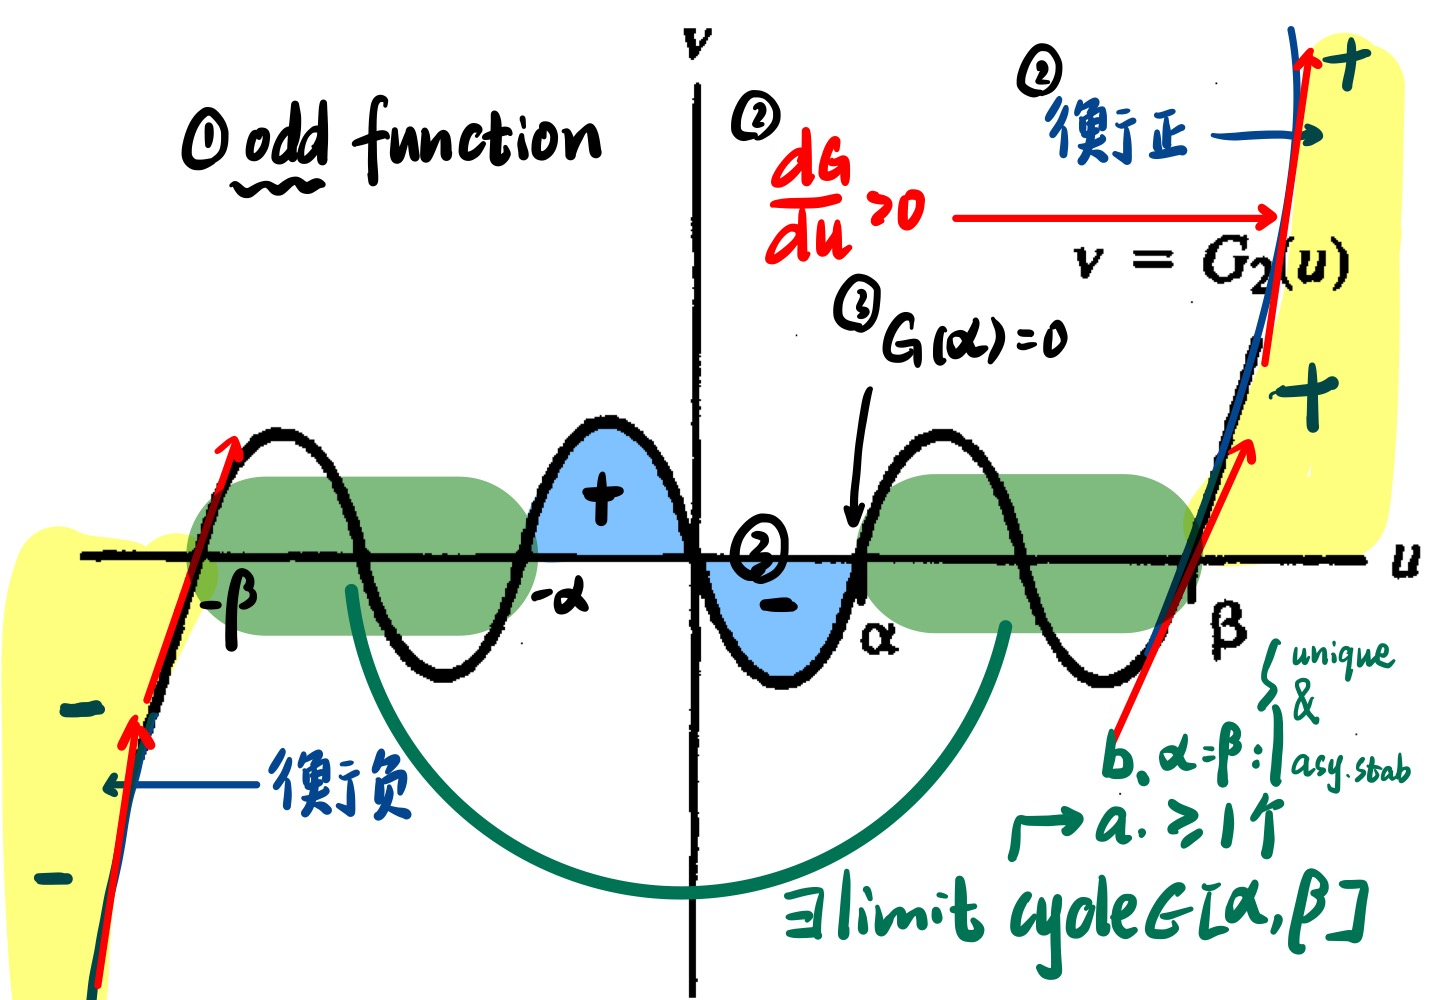
\includegraphics[width=1\textwidth]{figure_1.jpg}
\end{minipage}
\hfill
\begin{minipage}{0.75\textwidth}
    \begin{MyTh}{Find Limit Cycle}
        For $\left\{\begin{smallmatrix}\dot{u}=v-G(u) \\ \dot{v}=-u \quad \ \ \ \end{smallmatrix}\right.$ \ \ $\Leftrightarrow$ \ \ {\scriptsize $\frac{d^2u}{dt^2}+g(u)\frac{du}{dt}+u=0$ \ \ with $G(u)=\int^u_0 g(s)ds$. \quad \ps{Lienard Equations}} If we have:
        
        {\scriptsize \quad \tiny \ok{1}: $G(-u)=-G(u)$ \ps{(odd)} \quad \ok{2}: $\exists \alpha>0$ s.t. $G(\alpha)=0$ and $G(u)<0, \forall u\in(0,\alpha)$ \quad \ok{3}: $\exists \beta\geq\alpha$ s.t. $G(u)>0, \frac{dG}{du}>0, \forall u>\beta$ and $G(u)\to\infty$ as $u\to\infty$.}

        {\scriptsize \quad \ok{Then}: $G$ is `bumpy' function. \quad $^1$ $\exists$ limit cycle between $(\alpha,\beta),(-\beta,-\alpha)$. \quad $^2$ \ps{unique} and \ps{asy.stable} if $\alpha=\beta$}
    \end{MyTh}

    \begin{MyTh}{Relaxation Oscillations}
        A \ps{periodic} movement of \ps{``slow-fast alternation''}. {\scriptsize e.g. For $\left\{\begin{smallmatrix} \eps\dot{u}=v-G(u) \\ \dot{v}=-u \ | \ -u\eps \end{smallmatrix}\right.$ or More general form: $\left\{\begin{smallmatrix} \eps\dot{u}=f(u,v) \\ \dot{v}=g(u,v) \end{smallmatrix}\right.$} \ps{$|\eps|\ll1$}

        \begin{minipage}{0.2\textwidth}
            
\includegraphics[width=1\textwidth]{figure_2.jpg}
        \end{minipage}
        \hfill
        \begin{minipage}{0.8\textwidth}
            \ok{Relaxation Oscillations requies unstable equilibrium point.}

            \ok{Explain why it occur}: {\tiny $^1$ Find \textit{nullclines} (一般:直线+$S$曲线) $^2$ Since $\dot{u}=\frac{\text{some func}}{\eps}\gg 1$ (so that $|\dot{u}|\gg|\dot{v}|$) unless close to nullcline $\to$(一般$S$曲线) $^3$ 图上选4个点ABCD (只是一个示例而已),一般选S的local max/min加S更远处两个点, 连接成一个loop.
            $^4$判断ABCD点的流向 (看nullcline两侧/上下) $^5$分段分析 + \ps{从一不在nullcline上的点分析} e.g.$A\to B$ $\dot{u}=0$,$\dot{v}=-u<0$ 向下,慢阶段. $B\to C$ not close to S curve, $|\dot{u}|\gg1$ 向左,快阶段/\ps{fast horizontal jump}. $C\to D$ ... $D\to A$ ...}
        \end{minipage}
    \end{MyTh}
\end{minipage}

{\scriptsize \quad \ok{Estimate period $T$}: 例如上图 \scalebox{0.8}{\ps{\tiny (例子忽略了快反应)}} $T=\int_{t_A}^{t_B}dt+\int_{t_C}^{t_D}dt=2\int_{t_A}^{t_B}dt$ \ \ \ok{Find $dt=\_ du$ 带入计算} e.g. \scalebox{0.8}{\tiny In slow time: $\dot{u}=0\to v=G(u)$ and $\dot{v}=-u\to\frac{dv}{dt}=\frac{dv}{du}\frac{du}{dt}=G'(u)\frac{du}{dt}=-u\to -\frac{G'(u)}{u}du=dt$,带入计算}}

\begin{minipage}{0.17\textwidth}
    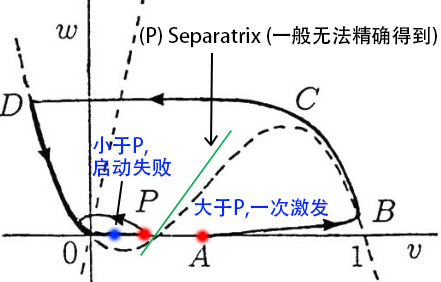
\includegraphics[width=1\textwidth]{figure_3.jpg}
\end{minipage}
\hfill
\begin{minipage}{0.83\textwidth}
    \begin{MyTh}{Excitable System}
        \ok{FitzHugh-Nagumo Model} $\left\{\begin{smallmatrix}\frac{dx}{dt}=c[y+x-\frac{x^3}{3}+z(t)] \\ \frac{dy}{dt}=\frac{-x+a+by}{c}\end{smallmatrix}\right.$ \ \ \ps{\tiny ($x$: \ps{excitability} variable; $y$: \ps{recovery} variable; $z(t)$: \ps{external stimulus})}

        {\tiny \ok{Threshold} 现象: \ok{Small perturbation}: return to equilibrium (\ps{failed initiation/excitation}). \quad \ok{Large perturbation}: large excursion before returning to equili. (\ps{action potential}|successful initiation).
        After excitation|大扰动之后: \ps{Refractory Period}不应期: system is unresponsive to further stimulation. \quad \ok{constant stimulus}: \ps{periodic firing} (limit cycle).
        
        \ok{Reason}: 寻找$\dot{u},\dot{v}$ s.t. $\ll,\gg 1$ \ps{i.e. $|\dot{u}|\gg|\dot{v}|$ or $|\dot{u}|\ll|\dot{v}|$}}
        
        \begin{MyTh}{Switch Behaviour}
            \tiny \ok{从一个stable point 到另一个stable point.} \scalebox{0.8}{\ps{(前面excitable system|relaxation oscillation如有两stable points且画图分析(像relaxation oscillation那样分析)可得到)}}
        \end{MyTh}
    \end{MyTh}
\end{minipage}

\begin{MyTh}{描述话语example}
    \tiny \ok{快-慢震荡}: $^1$(\ps{option}) The equilibrium point $S$ is unstable between the two \textit{knees}/\textit{turnning points} of the $u$-nullcline/cubic-like curve. | \ps{or}: $S$ changes stability as it crosses the knees of the $u$-nullcline. \ \ $^2$ 图上标/简单解释拐点位置. \ \ $^3$ 证明$|u'|\gg1$\ps{(写成乘积形式判断)}或其他$\to$得快运动边. \ \ $^4$ Trajectories \textit{starting off} the $u$-nullcline \textit{repidly/quickly} approach \textit{left/right branch} of the $u$-nullcline, and then \textit{slowly move down/up}|\textit{crawl along} the $u$-nullcline due to $v'<0/>0$, and to \textit{upper/lower knee/turnning point} $^5$ At the knee/turnning point, the trajectory \textit{quickly jumps} to the \textit{right/left branch} of the $u$-nullcline, and then \textit{slowly moves up/down}|\textit{crawl along} the $u$-nullcline due to $v'>0/<0$. $^6$ And this process \textit{repeats periodically}, giving rise to a \textit{relaxation oscillation}.
    \ok{Excitable}: 类似的,分析 small perturbation \textit{above/below} equilibrium point $S$ -> 得\textit{failed excitation} or \textit{successful excitation}.
\end{MyTh}


\section{Manifolds \& Fenichel's Theorem | SIR Model}

\begin{MyTh}{Regular/Singular Perturbation}
    {\scriptsize 对于一个含 $\eps$ 的方程/系统: \ \ If $\eps\to0$ the \ps{order} does not change, it's a \ok{regular perturbation}. \ \ If $\eps\to0$ the \ps{order} changes, it's a \ok{singular perturbation}.}

    \scalebox{0.94}{\tiny \ok{Find Roots}: Assume roots $x=x_0+\eps x_1+\eps^2 x_2+\cdots$, 代入比较$\Ocal(1),\Ocal(\eps)$...得系数\ps{\tiny (解前两系数就行)}.  \quad If \textit{singular}, cannot approx $x=\Ocal(\eps^{-1})$, rescaling $x=\frac{X}{\eps}$, assume root $X=X_0+\eps X_1+\cdots$ 类似前. 不留$X_0=0$解,因为X小.}

    \scalebox{0.94}{\tiny \ok{Sol \& Uniform}: 对$\eps \ddot{y}+p(x)\dot{y}+q(x)y=r(x)$, a.类似上面算sol \scalebox{0.8}{\ps{\tiny (有初值)}} or b.直接算exact sol. $\to$ 得\ok{Outer Solution} \scalebox{0.8}{\ps{\tiny (首项含$\eps$)}}. \quad Let $\tau=\eps t$ 类似算sol $\to$ \ok{Inner Solution} \scalebox{0.8}{\ps{\tiny (首项不含$\eps$)}}. \ \ \ok{unif expre} = Outer + Inner - Matching\scalebox{0.8}{\ps{(=matching cond 的lim)}}}
\end{MyTh}

\begin{MyTh}{Singular Perturbation System}
    \footnotesize For $\left\{\begin{smallmatrix}\dot{u}=f(u,v,\eps) \ \ \\ \dot{v}=\eps g(u,v,\eps)\end{smallmatrix}\right.$, \ps{\scriptsize $0<\eps\ll1$}. \quad If $\tau=\eps t$, then $\left\{\begin{smallmatrix}\eps u' =f(u,v,\eps) \\ \ \ v' =g(u,v,\eps) \end{smallmatrix}\right.$ \ \ \ps{$t$: fast time; $\tau$: slow time} \ \ \ps{\tiny ($\eps\ne0$时等价)} \qquad\qquad \ \ \ps{\tiny $\downarrow$ Defined in a neighborhood of $\mathcal{M}_0$}

    \quad {\scriptsize \ok{Reduced Problem}: slow times $\eps=0$. \ \ \ok{Layer Problem}: fast time $\eps=0$. \quad \ok{Critical Manifold}: $\mathcal{M}_0:=\{(u,v):f(u,v,0)=0\}$ \ \ \ps{\tiny ps: \textit{Reduced problem} defined only on $\mathcal{M}_0$, \textit{Layer problem} defined off $\mathcal{M}_0$}}

    \quad {\scriptsize \ok{Normal Hyperbolicity}: $\mathcal{M}_0$ is normally hyperbolic at $(u,v)\in\mathcal{M}_0$ if: \ \ $\lambda_i$ {\tiny (特征值)} of Jacobian $J|_{(u,v,0)}=\frac{\partial f}{\partial u}|_{(u,v,0)}$ are $\Re(\lambda_i)\ne0$. \ \ $\rightarrow$ \ \ \ok{(Un-)Stable}: $\Re(\lambda_i)<0$\scalebox{0.8}{\tiny $(>0)$}$\Leftrightarrow \frac{\partial f}{\partial u}<0$\scalebox{0.8}{\tiny $(>0)$} \scalebox{0.8}{\ps{\tiny (1-dim)}} }

    \quad {\scriptsize \ok{Outer Solution}: sol for slow time at $\eps=0$. (reduced problem) \quad \ok{Inner Solution}: sol for fast time at $\eps=0$. (layer problem)} \qquad\qquad\qquad\quad \ps{$\uparrow$ attracting(stable) / repelling(unstable)}

    \quad {\scriptsize \ok{Describe Reduced|Layer Problem}: \tiny $^1$ 如果能解具体表达式就解;不好解情况下给出$u',v'$仅关于$u,v$的表达式; $^2$ 如果可以画一个图; $^3$ 分析attracting/repelling (stable/unstable); $^4$ 分析$\tau,t\to\infty$时的行为}
\end{MyTh}

\begin{MyTh}{Fenichel's Theorem}
    If $\mathcal{M}_0\subset \{f(u,v,0)=0\}$ is \ps{compact} {\tiny (closed \& bounded)} and \ps{normally hyperbolic}. Suppose $f,g$ are \textit{smooth}. \ \ Then for $\eps>0$ \ps{\tiny (sufficiently small)}, $\exists$ \textit{Manifold} $\mathcal{M}_\eps$ s.t. \ps{$\Ocal(\eps)$ close} and \ps{diffeomorphic} to $\mathcal{M}_0$. (i.e. $\mathcal{M}_\eps$ is \ps{locally invariant} under the flow of the full system \ps{\tiny (上面左边的system)}). \quad \ps{\tiny ps: $M_\eps$ called \ok{slow manifold}.}

    \quad {\scriptsize \ok{Find $\mathcal{M}_\eps$}: If $\mathcal{M}_0=\{(u,v):u=p_0(v)\}$, then $\mathcal{M}_\eps=\{(u,v):u=p_{\eps}(v)\}$ \quad \scalebox{0.9}{\ps{\tiny 可通过算$u,v$的exact sol, 寻找能使含$t$项消失但保留$\tau$的解(or:考虑快变量$t\to\infty$), 对比$\mathcal{M}_0$得到$\mathcal{M}_\eps$}}}
    
    \quad {\scriptsize \ok{Invariance of Manifold}}: {\tiny For slow $M_{\eps}$|$M_0$ $\to$ manifold 中的等式关系$u=p(v)$两边对$\tau$|$t$求导 $\to$ 代入 slow|fast 对应的$u',v'$; 代入$M_{\eps}|M_0$中的等式关系 $\to$ 判断是否LHS=RHS.}
\end{MyTh}

\begin{MyTh}{SIR}
    {\scriptsize \ps{S}: \# people who are susceptible. {\tiny (易感人群)} \ \ \ps{I}: \# people who are infected. {\tiny (感染者)} \ \ \ps{R}: \# people who have been infected and recovered. {\tiny (no longer susceptible)}. {\tiny (康复者)} \ \ \ok{Total Pop}: $N=S+I+R$}

    \quad {\scriptsize \ok{Model}: $S'=-\beta SI$, $I'=\beta SI-\alpha I$, $R'=\alpha I$, $S,I\geq0$. \ok{Assumptions}: \scalebox{0.8}{\tiny $^1$ Mass Action incidence: $\beta N$ transmit infection/unit time; $^2$ $\alpha I$ recover/unit time; $^3$ No im/emigration, births, deaths. $^4$ No deaths from disease. $\to$ 新感人数=$\beta SI$ rate.}}

    \quad {\scriptsize \ok{临界值}: if $S>\frac{\alpha}{\beta}$, $I$ $\uparrow$ 疾病爆发; If $S<\frac{\alpha}{\beta}$, $I$ $\downarrow$ 疾病消退. \ \ $\Rightarrow$ \ok{Basic Reproduction Number}: \scalebox{0.9}{\ps{\tiny (A threshold quantity)}} $R_0=\frac{\beta S_0}{\alpha}$ or \ok{$\frac{\beta N}{\alpha}$}, $^1$ $R_0>1$ epidemic occurs; $^2$ $R_0<1$ disease dies out.}

    \quad {\scriptsize $\cdot$ $I_{\infty}=\lim_{t\to\infty}I(t)=0$; $S_{\infty}=(S+I)_{\infty}>0$; \ok{$N=S_0+I_0$} \ \ \ok{Final Size Relation}: $\ln(\frac{S_0}{S_\infty})=\frac{\beta}{\alpha}[N-S_\infty]=R_0[1-\frac{S_\infty}{N}]$ \scalebox{0.8}{\ps{\tiny As $(S+I)'=-\alpha I$ $\to$ $N-S_\infty=\alpha\int_0^\infty I dt$; As $\frac{S'}{S}=-\beta I$ $\to$ $\ln(\frac{S_0}{S_\infty})=\beta\int_0^\infty I dt$}}}
    
    \quad {\scriptsize \ok{Attack Rate/Ratio}: $N-S_\infty$ {\tiny (\# people ever infected | 总感染人数 | \ps{Final size of epidemic})} \quad \ok{Orbits Sol}: \tiny $I(t)+S(t)-\frac{\alpha}{\beta}\log(S(t))=N-\frac{\alpha}{\beta}\log(S_0)$ \ok{Peak}: $I_{\max}$ when $S=\frac{\alpha}{\beta}$ $\leftrightarrow$ $I'=0$ \scalebox{0.8}{\ps{\tiny (代入前面得精确 $I_{\max}$)}}}

    \quad {\scriptsize \ok{Infective Period}: $=\frac{1}{\alpha}$ \quad \ps{\tiny 就\textit{减去的那一项}的常数倒数为特征时间尺度} \qquad \ps{\tiny ps: e.g.可以由此计算单位时间内新感染人数(从开始): $\int_0^{\alpha^{-1}} I' dt=I(\alpha^{-1})-I(0)$}}
\end{MyTh}

\section{Reaction Diffusion}

\begin{MyTh}{Diffusion}
    \scriptsize Net movement from high to low concentration through random, small-scale motion.
\end{MyTh}
\begin{MyTh}{Fickian Diffusion}
    \scriptsize $J=-D\frac{\partial c}{\partial x}$ \ \ \ps{\tiny ($J$: flux; $D$: diffusivity; $c$: concentration; $-$: from high to low)}
\end{MyTh}

\vspace{-2pt}
\begin{MyTh}{Conservation Realtion}
    \tiny $\frac{\partial}{\partial t}\int_{x_0}^{x_1} c(x,t)dx=J(x_0,t)-J(x_1,t)$ \ps{\tiny $x_1=x_0+\Delta x$} \ \ When $\Delta x\to0$ $\Rightarrow$ $\frac{\partial c}{\partial t}=-\frac{\partial J}{\partial x}=$\scalebox{0.9}{$\frac{\partial (D\frac{\partial c}{\partial x})}{\partial x}$} \scalebox{0.9}{\ps{\tiny (If $D$ const. Heat Equation)}}
\end{MyTh}

\vspace{-5pt}
\begin{MyTh}{Solve PDE}
    {\tiny For $u(\mathbf{x},t)$,$\mathbf{x}=(x_1,\ldots,x_n)$; $u_t=D\Delta u$ with $u(\mathbf{x},0)=f(\mathbf{x})$ \quad If $f(\mathbf{x})=Q\delta(\mathbf{x})$, then \ok{Fundamental Sol}: \scalebox{0.9}{\tiny $u(\mathbf{x},t)=\phi(\mathbf{x},t)=\frac{Q}{(4\pi Dt)^{n/2}}e^{-\frac{|\mathbf{x}|^2}{4Dt}}$} \quad Else: \ok{General Sol}: $u(\mathbf{x},t)=\int_{\mathbb{R}^n} \phi(\mathbf{x}-\mathbf{y},t)f(\mathbf{y})d\mathbf{y}$}

    \vspace{-4pt}
    \quad {\scriptsize Moreover, for $u(\mathbf{x},t)$, $u_t=D\Delta u+a(t)u$ with $u(\mathbf{x},0)=f(\mathbf{x})$ \ \ $\Rightarrow$ \ \ $u(\mathbf{x},t)=v(\mathbf{x},t)e^{\int_0^t a(s)ds}$ with $v(\mathbf{x},0)=f(\mathbf{x})$ satisfying $v_t=D\Delta v$. \ \ $\to$ Use above. \qquad \ps{\tiny \ok{invades const. radial speed}: 算$\frac{dr}{dt}$}}
\end{MyTh}

\begin{MyTh}{Boundary}
    \tiny $^1$ \ok{\tiny Diffusion Model: 认为 $u(\mathbf{x},t)$ 是 \ok{bounded} 的} \ps{\tiny (travelling wave 不一定)} \scalebox{0.85}{\ps{\tiny (含$\pm\infty$, 极坐标$r\to\infty$, 得IC)}} \ \ $^2$ 对 $u$, $J$ \scalebox{0.85}{(flux)}, 有 \ok{continuous}. \scalebox{0.85}{\ps{\tiny (得BC,尤其是分段函数)}} \ \ $^3$ 对 $J$ \scalebox{0.85}{(flux)}, 考虑由物理意义, 边界\ps{\tiny 是否为0}
\end{MyTh}

\begin{MyTh}{假设和默认}
    \tiny $^1$ 若要假设$u(\mathbf{x},t)$的IC,考虑 $u(\mathbf{x},0)=b_0>0$ \scalebox{0.85}{\ps{\tiny (均匀的分布)}} \ \ $^2$ \imp{Stationary|Steady-state|Static}: $u_t=0$. \ \ $^3$ \imp{Homogeneous Rest State|Const. Equilibrium|Uniform Steady State}: $u_{\mathbf{x}}=0$ and $u_t=0$.
\end{MyTh}

\begin{MyTh}{Useful Tools}
    \tiny $^1$\ok{最后,可通过两边对$\mathbf{u}$对$\mathbf{x}$积分得待定系数值} \ \ $^2$ \ok{Linearise at $u^*$}: Let $u=u^*+\eta$, $|\eta|\ll1$ func. \ \ $^3$ 对于求解PDE, 考虑\ps{\tiny 直接计算} or \ps{\tiny Seperation of var.} \ \ $^4$ \ok{Desingularise}: e.g. For $u(x,t)$, Let $\tau=u t$
\end{MyTh}


\section{Travelling Waves}

\begin{MyTh}{Travelling Wave}
    {\scriptsize $u(x,t)=u(x-ct)=U(z)$ with $z=x-ct$. \ \ \ps{$c$: wave speed; $z$: wave variable} \ \ If $z=x-ct$ \textit{constant}, then $u$ \textit{constant}. \ \ \imp{Equilibrium}: 对于时间的求导为0, $u_t=0$}

    \vspace{-2pt}
    \quad {\scriptsize \ok{Condition}: For \ps{travelling wave under reaction-diffusion|\ok{wavefront}}, have $u(\pm\infty,t)=u^{\pm}$, and $u_x(\pm\infty,t)=0$ or $\lim_{z\to\pm\infty} U'(z)=\lim_{z\to\pm\infty} V(z)=0$ \quad {\tiny \imp{Spatially Homogeneous}: $u_{\mathbf{x}}=0$}}

    \vspace{-2pt}
    \quad {\scriptsize If $u(x,t)=U(z),z=x-ct$ and $u_t=f(u)+D u_{xx}$ \ \ $\Rightarrow$ \ \ Change to \ok{ODE: $-c U' = f(U) + D U''$} \ \ $\Rightarrow$ By using \ok{$V=U'$} $\to$ ODE System: $\left\{\begin{smallmatrix} U' = V \qquad\qquad \ \ \\ V' = -\frac{c}{D} V - \frac{f(U)}{D} \end{smallmatrix}\right.$}

    \vspace{-1pt}
    \quad {\scriptsize For $\uparrow$ travelling wave \ok{boundary conditions}: $U(-\infty)=u^-$ \ps{\tiny (ahead of wave)}; $U(\infty)=u^+$ \ps{\tiny (behind wave)} \ok{Heteroclinic orbit}: A trajectory connecting $(u^-,0)$ and $(u^+,0)$ \ps{\tiny (\ok{Homoclinic Orbit}:$u^-=u^+$)}}

    \quad {\scriptsize \ok{证明异宿轨道存在}: {\tiny Using $\frac{dU}{dV}=\frac{U'}{V'}$ to find \ok{$V(U)$}. If $V(u^{\pm})=0$, then \ps{exists}.} \ \ \ok{寻找波速$c$}: {\tiny Find ODE: $DU''+cU'+f(U)=0$ \ $\to$ \ 乘$U'$两边积分: $D\int_{-\infty}^{\infty} U'' U' dz+c\int_{-\infty}^{\infty} (U')^2 dz+\int_{-\infty}^{\infty} f(U)U' dz=0$}}

    \vspace{-3pt}
    \quad {\scriptsize $\updownarrow$ \ps{show: reasonable exist $u$ s.t. $\lim_{z\to\pm\infty} u(z)=u^{\pm}$ exists \quad || \quad}}{\scriptsize $\to$ using \ps{$U''U'=\frac{1}{2}[(U')^2]'$} $\to$ $\int_{-\infty}^{\infty}U''Udz=0$ and $U'dz=dU$ \ \ $\Rightarrow$ \ \ $c=[\int_{u^+}^{u^-} f(U)dU] \ / \ [\int_{-\infty}^{\infty} (U')^2 dz]$ \ps{\tiny (ps:$c$符号 \ 面积差决定)}}

    \begin{minipage}{0.88\textwidth}
        \quad {\tiny Find equilibrium: $V=0$ and $U_1,U_2,U_3$ \ $\to$ \ 计算 Jacobian + 判断 stability \ $\to$ \ 边上两saddle, 中间node/focus \ $\to$ \ \scalebox{0.85}{only interest in the unstable eigendirection} \ $\to$ \ps{\tiny 不用算/简短算出} $U_1,U_3$ 处的eigenvector 方向: 说明 $^1$一个方向进\ps{\tiny (stable eigendirection,特征值<0)}, 一个方向出\ps{\tiny (unstable eigendirection,特征值>0); $^2$左边进/出的方向(positive/negative slope), 右边出/进的方向(negative/positive slope). \ok{i.e. 有交点+一进一出}} \ $\Rightarrow$ possible for a heteroclinic connection between $U_1$ and $U_3$. \quad || \quad if $c=[\int_{u^+}^{u^-} f(U)dU] \ / \ [\int_{-\infty}^{\infty} (U')^2 dz]=0$, \ok{critical front speed} \ \ \scalebox{0.9}{\ps{\tiny 对于灾害:$c<0$ no spread; $c>0$ outbreak spread}}}
    \end{minipage}
    \hfill
    \begin{minipage}{0.12\textwidth}
        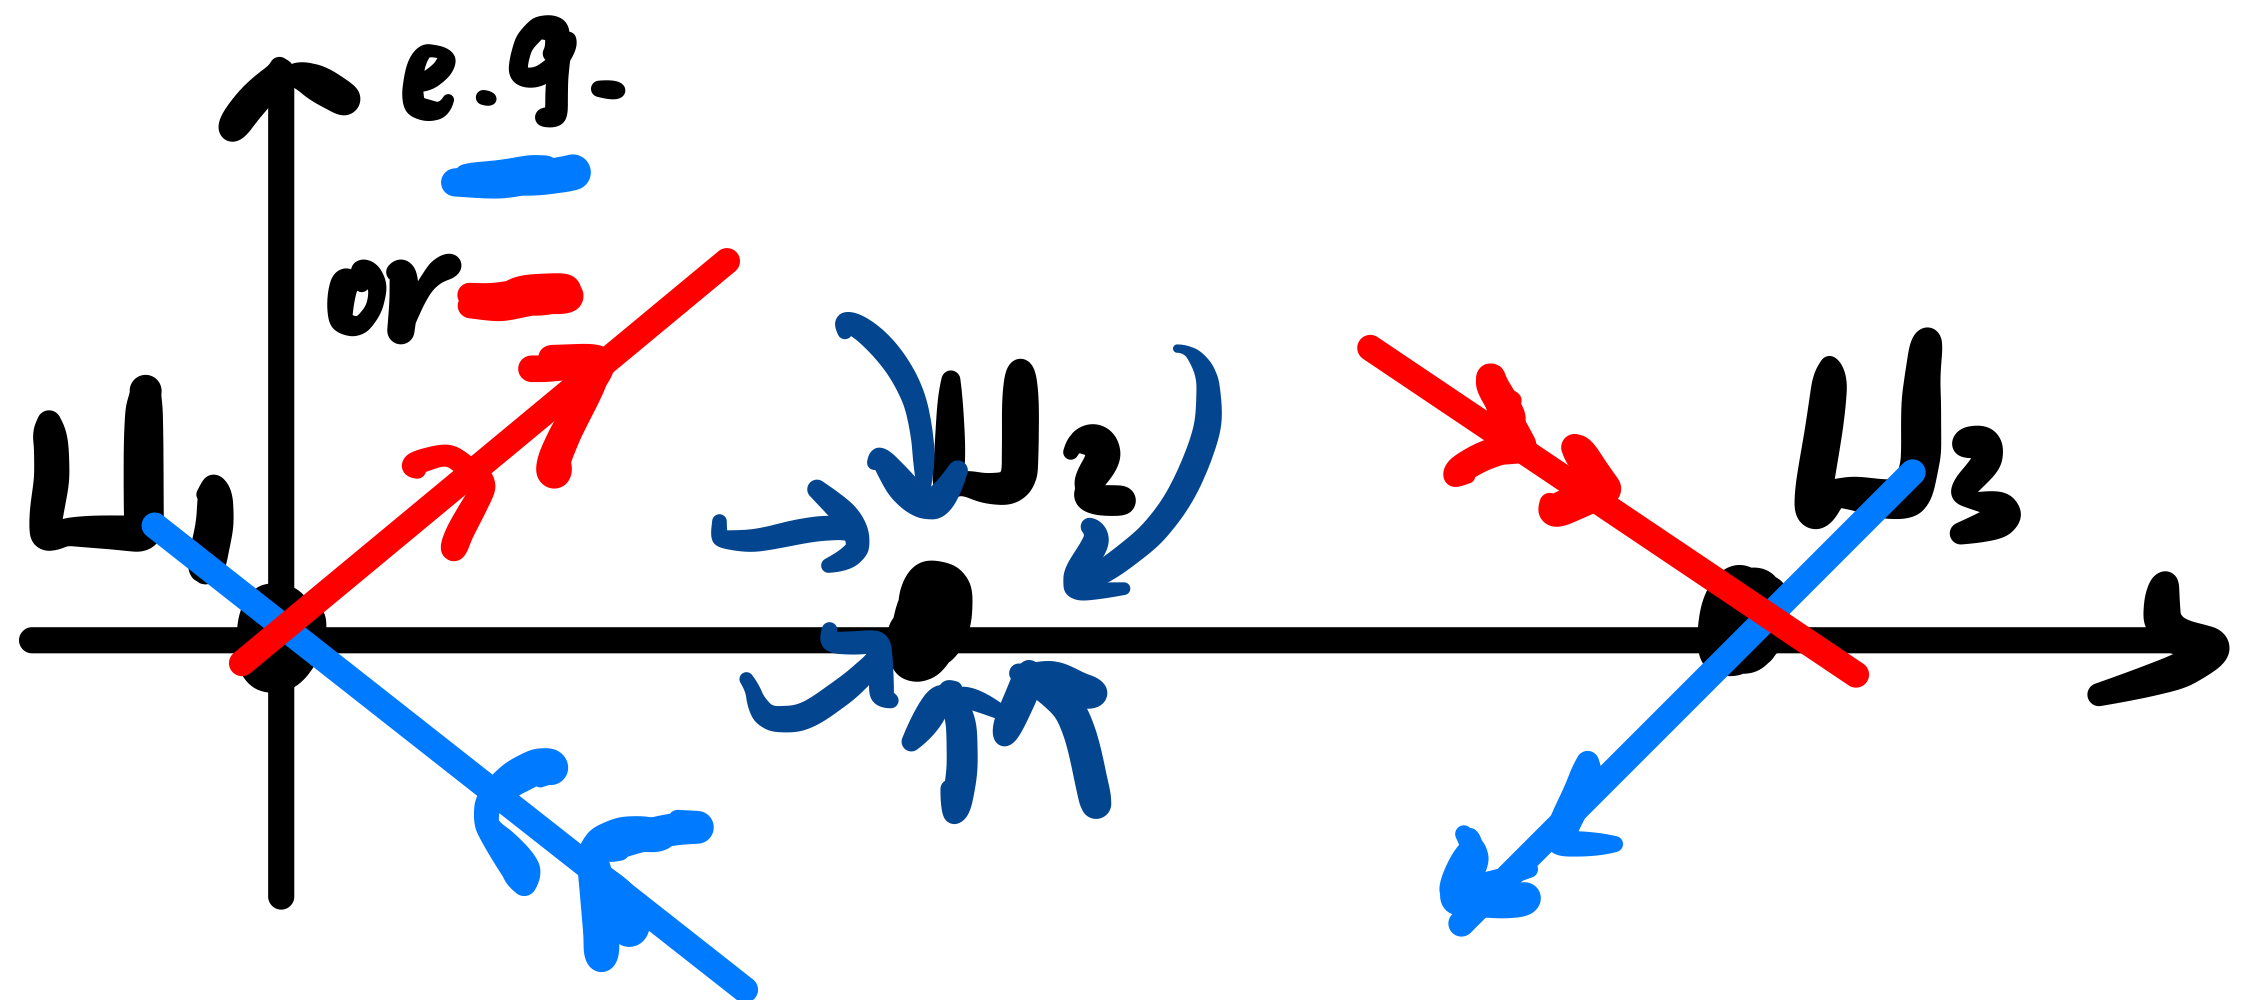
\includegraphics[width=1\textwidth]{figure_4.png}
    \end{minipage}
\end{MyTh}

\vspace{-4pt}
\begin{MyTh}{Fisher-Kolmogoroff}
    \tiny \textit{Eq}: $u_t=Du_{xx}+ru(1-\frac{u}{K})$ $\Leftrightarrow$ $U'' + \frac{c}{D} U' + \frac{r}{D} U(1-\frac{U}{K})=0$ when $u(x,t)=U(z),z=x-ct$. \ \ \ok{如有wavefront sol:} \ok{Wave Speed}: $c\geq c_{\min}=2$, and $\lim_{z\to-\infty|\infty} U(z)=K|0$.
\end{MyTh}

\begin{MyTh}{Remark}
    \scriptsize \ok{1.} 对于单 PDE/ODE 中, Equilibrium 的稳定性判断看$f'(u^*)$ 符号; 对于 ODE System 中, 看 Jacobian. \ps{\tiny (两者不同)} \ \ \ok{2.} $u(x,t)$ 如用\ok{Seperation of var.}算出$x=$const. 要wave sol时忽略.
\end{MyTh}

\begin{MyTh}{For $\lambda=0$ Case|Degenerate}
    \tiny 判Stability时如特征值为: $\lambda_1=0,\lambda_2<0$: It's a "saddle-node" with one stable eigendirection (corresponding to $\lambda_2<0$) and one "center" eigendirection (corresponding to $\lambda_1=0$).
\end{MyTh}


\section{Appendix}

\tiny

\begin{MyTh}{$y'+p(x)y=q(x)$}
    \ok{Integrating Factor}: $I(x)=e^{\int p(x)dx}$ \ \ $\Rightarrow$ \ \ $I(x)y=\int I(x)q(x)dx$
\end{MyTh}
\begin{MyTh}{Taylor Expansion}
    $f(x,r)$ at $(x_0,r_0)$: $f(x,r)=f(x_0,r_0)+(x-x_0)f_x|_{(x_0,r_0)}+(r-r_0)f_r|_{(x_0,r_0)}+\frac{1}{2}\cdots$
\end{MyTh}

\vspace{-2pt}
\begin{MyTh}{Binomial Series}
    $(1+x)^\alpha=1+\alpha x+\frac{\alpha(\alpha-1)}{2!}x^2+\cdots$ \quad
\end{MyTh}
\begin{MyTh}{Linerisation}
    $f(x+\Delta x)=f(x)+f'(x)\Delta x+\cdots$ \quad $e^{bx}=1+bx+\frac{(bx)^2}{2!}+\cdots$ \quad $\ln(a+x)=\ln(a)+\frac{x}{a}-\frac{x^2}{2a^2}+\frac{x^3}{3a^3}-\cdots$ \quad $y(a)-y(b)=\int_b^a y'(x)dx$
\end{MyTh}

\vspace{-2pt}
\begin{MyTh}{Geometry Series}
    $\frac{1}{1-x}=1+x+x^2+\cdots$, $|x|<1$
\end{MyTh}
\begin{MyTh}{Hyperbolic Funcs}
    $\sinh x=\frac{e^x-e^{-x}}{2}$ \ \ $\cosh x=\frac{e^x+e^{-x}}{2}$ \ \ $\tanh x=\frac{\sinh x}{\cosh x}$ \quad $\sinh(x)=x+\frac{x^3}{3!}+\frac{x^5}{5!}+\cdots$ \ \ $\cosh(x)=1+\frac{x^2}{2!}+\frac{x^4}{4!}+\cdots$ \ \ $\tanh(x)=x-\frac{x^3}{3}+\frac{2x^5}{15}-\cdots$
\end{MyTh}

\vspace{-2pt}
\begin{MyTh}{Integral}
    $\text{arctanh}(x)=\frac{1}{2}\ln\left(\frac{1+x}{1-x}\right)$ \ \ $\text{arcsinh}(x)=\ln\left(x+\sqrt{x^2+1}\right)$ \ \ $\text{arccosh}(x)=\ln\left(x+\sqrt{x^2-1}\right)$ \quad $\int \frac{1}{\sqrt{a^2-x^2}}dx=\arcsin(\frac{x}{a})$ \ \ $\int \frac{1}{a^2+x^2}dx=\frac{1}{a}\arctan(\frac{x}{a})$
\end{MyTh}

\vspace{-2pt}
\begin{MyTh}{Useful Tools}
    $\Delta u=u_{xx}+u_{yy}=u_{rr}+\frac{1}{r}u_r+\frac{1}{r^2}u_{\theta\theta}$
    \quad If $u$ \ok{radial symmetry}: $u=u(r,t)$ (i.e. $u_\theta=0$)
    \quad \ok{$dA=rdrd\theta$ in polar coord.} and \ok{$dV=r^2\sin\phi dr d\theta d\phi$ in spherical coord.}
\end{MyTh}

\vspace{-2pt}
\begin{MyTh}{$ay''+by'+cy=0$}
    \ok{$y''-\lambda y=0$}: \ \ $^1$ $\lambda>0$: $y=C_1\cosh(\sqrt{\lambda}x)+C_2\sinh(\sqrt{\lambda}x)= A e^{\sqrt{\lambda}x}+B e^{-\sqrt{\lambda}x}$; \quad $^2$ $\lambda=0$: $y=C_1+C_2 x$; \quad $^3$ $\lambda<0$: $y=C_1\cos(\sqrt{-\lambda}x)+C_2\sin(\sqrt{-\lambda}x)$

    \quad \ok{General}: \textit{characteristic eq.}: $a r^2 + b r + c = 0$, root $r_{1,2}=\mu\pm\nu i$. \quad $^1$ $\Delta>0$: $y=C_1 e^{r_1 x}+C_2 e^{r_2 x}$; \quad $^2$ $\Delta=0$: $y=e^{\mu x}(C_1+C_2 x)$; \quad $^3$ $\Delta<0$: $y=e^{\mu x}(C_1\cos(\nu x)+C_2\sin(\nu x))$
\end{MyTh}

\vspace{-2pt}
\begin{MyTh}{Seperation of var.}
    $^1$ 假设 $u(x,t)=X(x)T(t)$ \ \ $\to$ 带入PDE $^2$ 解出类似 $\frac{T'}{DT}=\frac{X''}{X}=-\lambda$ $\to$ 得到两个ODE \ $^3$ 解较为简单的ODE, 代入BC解$\lambda$和sol. \ps{\tiny (注意看是否只要periodic; 极坐标有$r\to\infty$ bounded, $\theta=\theta+2\pi$等条件)}, $^4$ 解另外一个. \ $^5$ 叠加所有$\lambda_n$的sol得到PDE的general sol $u=\sum c_nX_n(x)T_n(t)$ \ $^6$ 用IC解出$c_n$. \qquad \ps{\tiny Remark: $^1$ 前期可以用正比化简; $^2$ $\lambda$ 为 让 sin/cos 解为正好计算.}
\end{MyTh}

\begin{MyTh}{Polar Coord.}
    $x=r\cos\theta$, $y=r\sin\theta$ \ $\to$ \ $2rr'=2xx'+2yy'$ and $r^2\theta'=xy'-yx'$  
\end{MyTh}



\end{document}